\documentclass[border=10pt]{standalone}
\usepackage{tikz}
\usepackage{amsmath}
\usetikzlibrary{arrows.meta, positioning, fit, backgrounds, calc, decorations.pathreplacing}

\definecolor{inputcol}{HTML}{4A90D9}
\definecolor{prepcol}{HTML}{5BAE5F}
\definecolor{timecol}{HTML}{E8913A}
\definecolor{freqcol}{HTML}{9B59B6}
\definecolor{fusioncol}{HTML}{E74C3C}
\definecolor{enccol}{HTML}{2980B9}
\definecolor{reccol}{HTML}{1ABC9C}
\definecolor{losscol}{HTML}{C0392B}

\begin{document}
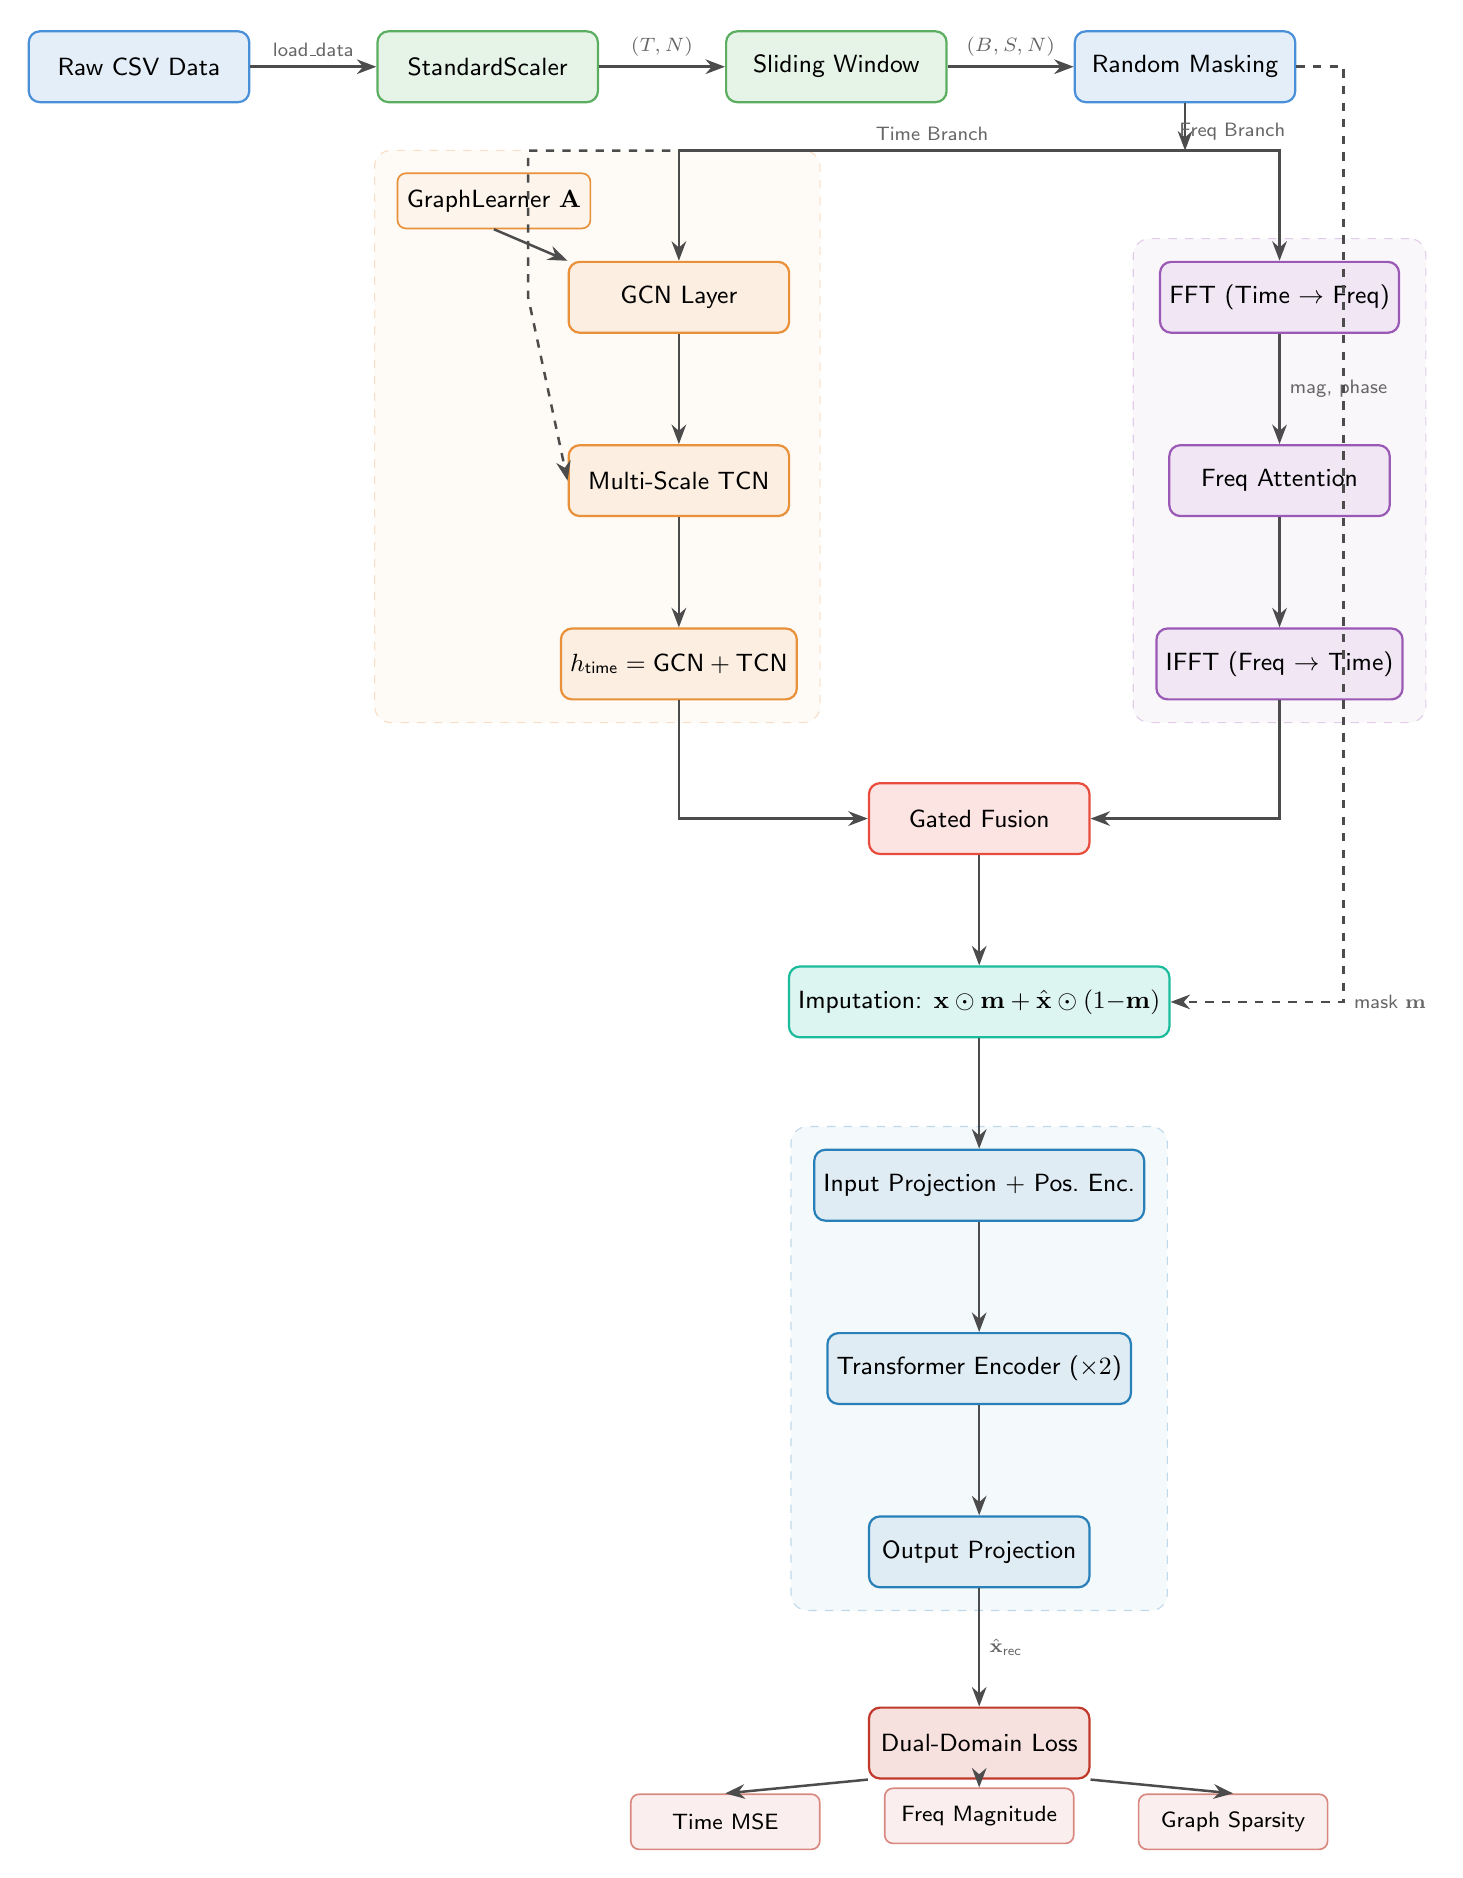
\begin{tikzpicture}[
    >=Stealth,
    node distance=1.4cm and 1.6cm,
    every node/.style={font=\sffamily\small},
    block/.style={
        draw, rounded corners=4pt, minimum width=2.8cm, minimum height=0.9cm,
        text centered, font=\sffamily\small, line width=0.8pt
    },
    smallblock/.style={
        draw, rounded corners=3pt, minimum width=2.4cm, minimum height=0.7cm,
        text centered, font=\sffamily\footnotesize, line width=0.6pt
    },
    arrow/.style={->, line width=0.9pt, color=black!70},
    darrow/.style={->, line width=0.9pt, color=black!70, dashed},
    label/.style={font=\sffamily\scriptsize, text=black!60},
]

% ===== Row 1: Input & Preprocessing =====
\node[block, fill=inputcol!15, draw=inputcol] (csv) {Raw CSV Data};

\node[block, fill=prepcol!15, draw=prepcol, right=of csv] (scaler) {StandardScaler};

\node[block, fill=prepcol!15, draw=prepcol, right=of scaler] (window) {Sliding Window};

\node[block, fill=inputcol!15, draw=inputcol, right=of window] (masking) {Random Masking};

% ===== Row 2: Dual Branches (below masking, centered) =====
% Time branch
\node[block, fill=timecol!15, draw=timecol, below=2.0cm of window, xshift=-2.0cm] (gcn) {GCN Layer};
\node[smallblock, fill=timecol!10, draw=timecol, above left=0.4cm and -0.3cm of gcn] (graphlearn) {\small GraphLearner $\mathbf{A}$};
\node[block, fill=timecol!15, draw=timecol, below=of gcn] (tcn) {Multi-Scale TCN};
\node[block, fill=timecol!15, draw=timecol, below=of tcn] (timesum) {$h_{\text{time}} = \text{GCN} + \text{TCN}$};

% Freq branch
\node[block, fill=freqcol!15, draw=freqcol, below=2.0cm of masking, xshift=1.2cm] (fft) {FFT (Time $\to$ Freq)};
\node[block, fill=freqcol!15, draw=freqcol, below=of fft] (attn) {Freq Attention};
\node[block, fill=freqcol!15, draw=freqcol, below=of attn] (ifft) {IFFT (Freq $\to$ Time)};

% ===== Row 3: Fusion =====
\node[block, fill=fusioncol!15, draw=fusioncol,
      below=1.5cm of $(timesum)!0.5!(ifft)$] (fusion) {Gated Fusion};

% ===== Row 4: Imputation =====
\node[block, fill=reccol!15, draw=reccol, below=of fusion] (impute)
     {Imputation: $\mathbf{x} \odot \mathbf{m} + \hat{\mathbf{x}} \odot (1{-}\mathbf{m})$};

% ===== Row 5: Transformer Encoder =====
\node[block, fill=enccol!15, draw=enccol, below=of impute] (proj) {Input Projection + Pos.\ Enc.};
\node[block, fill=enccol!15, draw=enccol, below=of proj] (transf) {Transformer Encoder ($\times 2$)};
\node[block, fill=enccol!15, draw=enccol, below=of transf] (outproj) {Output Projection};

% ===== Row 6: Loss =====
\node[block, fill=losscol!15, draw=losscol, below=1.5cm of outproj] (loss)
     {Dual-Domain Loss};

% Loss sub-items
\node[smallblock, fill=losscol!8, draw=losscol!60,
      left=0.6cm of loss, yshift=-1.0cm] (ltime) {Time MSE};
\node[smallblock, fill=losscol!8, draw=losscol!60,
      below=0.1cm of loss, xshift=0cm] (lfreq) {Freq Magnitude};
\node[smallblock, fill=losscol!8, draw=losscol!60,
      right=0.6cm of loss, yshift=-1.0cm] (lsparse) {Graph Sparsity};

% ===== ARROWS =====
% Row 1 flow
\draw[arrow] (csv) -- (scaler) node[midway, above, label] {load\_data};
\draw[arrow] (scaler) -- (window) node[midway, above, label] {$(T, N)$};
\draw[arrow] (window) -- (masking) node[midway, above, label] {$(B, S, N)$};

% Split into two branches
\coordinate (splitpt) at ($(masking.south)+(0,-0.6)$);
\draw[arrow] (masking.south) -- (splitpt);
\draw[arrow] (splitpt) -| (gcn.north) node[pos=0.25, above, label] {Time Branch};
\draw[arrow] (splitpt) -| (fft.north) node[pos=0.25, above, label] {Freq Branch};

% Graph learner feeds adjacency to GCN
\draw[arrow] (graphlearn.south) -- (gcn.north west);

% Time branch internal
\draw[arrow] (gcn) -- (tcn) node[midway, right, label] {};
\draw[arrow] (tcn) -- (timesum);

% Also feed original x into TCN (parallel path)
\coordinate (tcndirect) at ($(gcn.west)+(-0.5, 0)$);
\draw[darrow] (splitpt) -| (tcndirect) -- (tcn.west);

% Freq branch internal
\draw[arrow] (fft) -- (attn) node[midway, right, label] {mag, phase};
\draw[arrow] (attn) -- (ifft);

% Branches to fusion
\draw[arrow] (timesum.south) |- (fusion.west);
\draw[arrow] (ifft.south) |- (fusion.east);

% Fusion onward
\draw[arrow] (fusion) -- (impute);

% Mask feeds into imputation (from masking, side path)
\coordinate (maskside) at ($(masking.east)+(0.6,0)$);
\draw[darrow] (masking.east) -- (maskside) |- (impute.east)
    node[pos=0.5, right, label] {mask $\mathbf{m}$};

\draw[arrow] (impute) -- (proj);
\draw[arrow] (proj) -- (transf);
\draw[arrow] (transf) -- (outproj);
\draw[arrow] (outproj) -- (loss) node[midway, right, label] {$\hat{\mathbf{x}}_{\text{rec}}$};

% Loss sub-items
\draw[arrow] (loss.south west) -- (ltime.north);
\draw[arrow] (loss.south) -- (lfreq.north);
\draw[arrow] (loss.south east) -- (lsparse.north);

% ===== Branch labels (background boxes) =====
\begin{scope}[on background layer]
    \node[fit=(gcn)(tcn)(timesum)(graphlearn),
          fill=timecol!5, draw=timecol!30, dashed, rounded corners=6pt,
          inner sep=8pt, label={[timecol, font=\sffamily\footnotesize]above:Time Branch}] {};
    \node[fit=(fft)(attn)(ifft),
          fill=freqcol!5, draw=freqcol!30, dashed, rounded corners=6pt,
          inner sep=8pt, label={[freqcol, font=\sffamily\footnotesize]above:Frequency Branch}] {};
    \node[fit=(proj)(transf)(outproj),
          fill=enccol!5, draw=enccol!30, dashed, rounded corners=6pt,
          inner sep=8pt, label={[enccol, font=\sffamily\footnotesize]left:Transformer Encoder}] {};
\end{scope}

\end{tikzpicture}
\end{document}
